%!TEX root = ../thesis.tex
%*******************************************************************************
%****************************** Third Chapter **********************************
%*******************************************************************************
\chapter{The Short-Baseline Near Detector and The Booster Neutrino Beam}

% **************************** Define Graphics Path **************************
\ifpdf
    \graphicspath{{Chapter3/Figs/Raster/}{Chapter3/Figs/PDF/}{Chapter3/Figs/}}
\else
    \graphicspath{{Chapter3/Figs/Vector/}{Chapter3/Figs/}}
\fi

%********************************** %Opening  **************************************

Chapter 3 Opening

\newpage

%********************************** %First Section  **************************************
\section{Liquid Argon Time Project Chambers Overview}

%1: Overview of LArTPC, why LArTPC and what LArTPC does
The Short-Baseline Near Detector (SBND) is a 112 t Liquid Argon Time Projection Chamber (LArTPC), designed for precise measurement of neutrino interactions from the Booster Neutrino Beam (BNB) at Fermilab.
LArTPC employs a liquefied medium of argon for neutrino detection, enabling extremely high spatial and calorimetry resolution as well as scaling detector to a large target mass.
Due to their excellent performance, LArTPC is a technology of choice for Fermilab's neutrino program, including the Short-Baseline Neutrino (SBN) program \cite{} (SBND, MicroBooNE and ICARUS experiments) and the upcoming Deep Underground Neutrino Experiment (DUNE) \cite{}.

%2: LArTPC description and figure 
A diagram depicting a general LArTPC can be seen in Fig. \ref{LARTPC}.
Particles resulting from a neutrino interaction ionise the argon as they traverse the detector medium.
A high negative voltage is applied at the cathode plane, creating an electric field under which the ionised electrons drift towards the anode.
The drifting electrons induce signals on the three readout wire planes located at the anode, yielding a high granularity image of the interaction.
Since the wire planes are transparent to the scintillation photons resulting from particles propagation inside liquid argon, an additional Photon Detection System (PDS) is located behind the wire planes.
The information from the photons gains precise timing information of the interaction.

\begin{figure}[h] 
\centering    
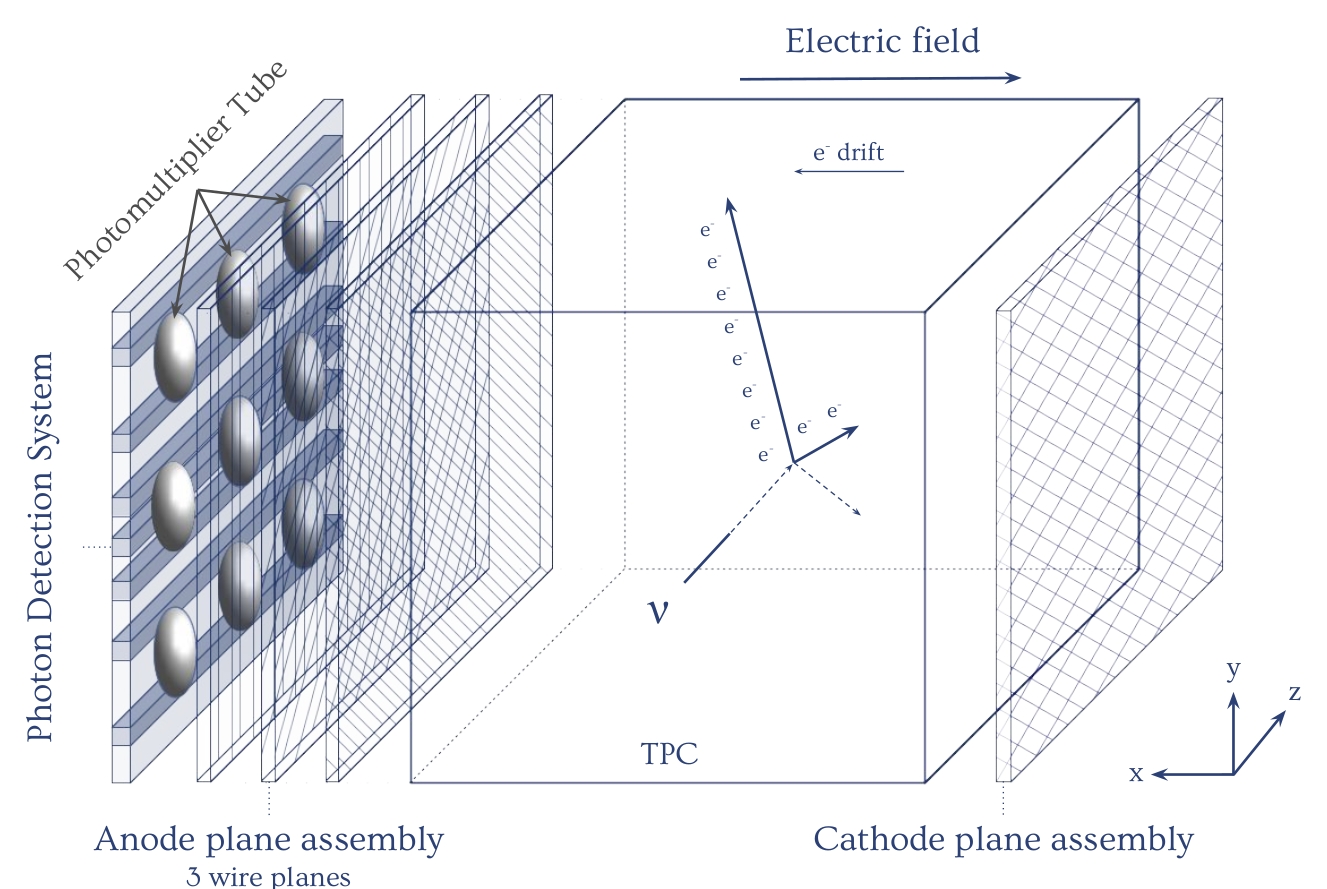
\includegraphics[width=1.0\textwidth]{LARTPC}
\caption[LARTPC]{
	Fig. from \cite{}.
}
\label{fig:LARTPC}
\end{figure}

This following section will delve into the details of operation principle of a LArPTC.
Sec. \ref{sec3:creation} provides the technical details of how a particle can ionise to produce drifting electrons, and then recombine to produce scintillation photons.
Sec. \ref{sec3:propagation} then describes how the produced drifting electrons and scintillation photons propagate across the liquid argon medium, and their detection is included in Sec. \ref{sec3:detection}.
Lastly, Sec. \ref{sec3:pid} explains how the measured signals can be used for calorimetry, and hence, particle identification.

\subsection{Ionisation, Scintillation and Recombination}
\label{sec3:creation}

\subsubsection{Ionisation}
%Ionisation
%Energy loss profile
Particles traversing a medium like liquid argon experience energy loss via ionisation, producing ionised electrons as secondary particles. 
The typical energy loss profile for particles is shown in Fig. \ref{}, specifically for a muon traversing in a copper medium but the principle is applicable to liquid argon.
This plot shows the stopping power,the energy loss per unit length divided by the density of the target medium, against the momentum of the traversing particle.
At the energy ranges relevant in LArTPC, heavy particles like muons, pions, and protons, lose energy as described by the Bethe-Block formalism.
For lighter and highly relativistic particles, such as > 100 MeV electrons and photons in liquid argon, the energy loss mechanism is primarily via radiative effects.
An example for both of these event topologies are shown in Fig. \ref{}.

%Track like
Muons, pions and protons traverse liquid argon and interact electromagnetically with its atom, primarily via Multiple Coulomb Scattering (MCS) and freeing electrons along their trajectories.
Since these trajectories are typically straightly lines, they are referred to as \textit{tracks}.
The MSC process is dependent on the particle momentum.
The energy deposited per unit length via ionisation, $dE/dx$, is typically constant in the Minimum Ionising Particle (MIP) but arises when the particle comes to a stop, called Bragg peak.
The energy loss profile is dependant on the particle mass, and thus often used to perform Particle IDentification (PID) \cite{}, most effective for protons separation from muons and pions.
The energy depositions for tracks in the MIP region is described a Landau-Gaussian Convolution (LCG), where the Most Probable Value (MPV) describes the most deposited region.

%Shower like
Electrons with energy above the critical energy, the energy at at which losses by ionisation are equal to losses by radiation, deposit energy via radiative effects.
This typically produce cones of electromagnetic activities, also known as \textit{showers}. 
The critical energy for electron in liquid argon is 32.8 MeV.
Photons are neutral particles and therefore can travel some distance without ionising and before depositing energy inside the liquid argon.
This produces a gap between the interaction vertex and the start of the shower, called \textit{conversion gap}.
This distance is plotted in Fig. \ref{}.
At low energies, photon lose energy primarily via Compton scattering but at higher energy, pair production is the dominating effects, producing an $e^{+}e^{-}$ pair.
Both the energy loss profiles and the conversion gaps can be used for distinguishing between electrons and photons (See Chap. \ref{}). 

\subsubsection{Scintillation}
%Scintillation light
Moreover, charged particles traversing liquid argon also produce scintillation photons as secondary particles, through two different processes that both result in an argon excimer ($Ar_{2}^{*}$) shown in Fig. \ref{}.
The first process is known as self-trapped exciton.
This begins with the charged particle does not have sufficient energy for ionisation, and hence, excites the argon atom upon collision instead.
The excited argon atom ($Ar^{*}$) self-traps with another argon atom, forming an argon excimer ($Ar^{*}_{2}$).
The second process is known as recombination.
Ionisation in liquid argon produce a free electron and an argon ion ($Ar^{+}$).
The electron can either escape and drift towards the anode for detection, or recombine with an argon ion and an argon atom ($Ar$), forming an argon excimer ($Ar_{2}^{*}$).

The argon excimer is short-lived and undergoes radiative decay into two ground-state argon atoms, producing scintillation photons with wavelength of 128 nm in the Vacuum UltraViolet (VUV) range \cite{}.
The timing constant of the decay depends on the excitation state.
The singlet state has a shorter mean lifetime with a decay constant $\tau_{S} \approx 6$ ns, while the triplet has a longer mean lifetime with a decay constant $\tau_{T} \approx 1.5$ $\mu$s.
The time-dependent probability of light emission in pure liquid argon can therefore be modelled as
\begin{equation}
	l(t)=\frac{A_{S}}{\tau_{s}}\exp{\left(-\frac{t}{\tau_{s}}\right)} +\frac{A_{T}}{\tau_{T}}\exp{\left(-\frac{t}{\tau_{T}}\right)}
\end{equation}
where $A_{S}$ and $A_{T}$ are the decay amplitudes of the singlet and triplet states respectively. For a MIP muon, the ratio of singlet-to-triplet state is $\approx 1:3$, where $A_{S} \approx 0.25$ and $A_{T} \approx 0.75$ \cite{}.

%Quenching
Liquid argon is an excellent medium to produce scintillation light, emits about 20000 photons per MeV of deposited energy at 500 V/cm \cite{}.
However, the number of emitted photons are subject to quenching.
Quenching can be caused by ionisation density \cite{} or contaminants in the liquid argon such as oxygen and nitrogen absorb the energy without emitting any photons \cite{}.

\subsubsection{Recombination}

%Recombination

The electron-ion recombination, one of the two processes to produce scintillation photon, occurs immediately within 1-2 ns following the electron ionisation process.
As shown in Fig. \ref{}, the resulting number of ionisation electrons and photons are anti-correlated, driven by the recombination $R$ 
\begin{equation}
	R=W_{ion} \cdot \frac{dE/dx}{dQ/dx}
\end{equation}
where $W_{ion} = 23.6$ eV is the energy required to ionise and argon and $\frac{dQ}{dx}$ and $\frac{dE}{dx}$ is the charge and energy loss per unit length respectively \cite{}. 
If not taken into account, the recombination can result in underestimating energy loss due to ionisation.

A popular model to describe this effect is the Box Model \cite{}, which the inverse Box Model equation is modelled as \cite{}
\begin{equation}
	\frac{dE}{dx} = \frac{1}{\beta}\left[ \exp{\left( \beta W_{ion}  \frac{dQ}{dx}\right)} -\alpha \right]
\end{equation}
where $\alpha$ and $\beta$ are tunable parameters.
Recombination is highly dependent on the electric field and the local charge density.
The effects of the electric field intensity is folded into the $\beta$ parameter.
ArgoNeuT experiment has recently measured the recombination factor in LArTPC \cite{}, and demonstrated a data-driven study on recombination factor.
The resulting ``Modified Box Model" with parameter $\alpha = 0.93$ and $\beta = 0.30 $ MeV/cm best describes the recombination effects in LArTPC.

\subsection{Electron Drift and Photon Propagation}
\label{sec3:propagration}

%Transportation of ionised electrons, diffusions, impurities

\subsubsection{Electron Diffusion}

%Electron drift under electric field
Ionised electrons that do not recombine are drifted towards the anodes under the effects of electric field, by applying a high negative voltage to the cathode.
Under the conditions of SBND with a drift field of 500 V/cm and a temperature of 87 K, the drift velocity of electrons is 0.16 cm/$\mu$s.

%diffusion
As the ionised electrons drift, they undergo diffusion, which perturbs the trajectory of the electrons due to various effects, such as inelastic collisions.
Diffusion causes the shape of of a cloud of electrons produced in a point like energy deposition to grow in volume while drifting.
The effects increase with respect to the drift distance and smear both spatial and temporal resolutions.

The Gaussian profile resulting from the response function of the charge deposition on the wire can therefore be modelled as 

\begin{equation}
	\sigma^{2} (t) = \sigma^{2}_{0} + \left(\frac{2D}{v^{2}_{d}}\right)t
\end{equation}
The observed profile $\sigma$ depends on the initial profile (no diffusion) $\sigma_{0}$, the drift velocity $v_{d}$, the drift time $t$ and the diffusion coefficient $D$ \cite{}.
Diffusion is parameterised in both longitudinal direction $D_{L}$ (parallel to the drift ad field direction) and transverse direction $D_{T}$ (perpendicular to the drift and field direction).
Longitudinal diffusion is due to individual electron arriving on the wire earlier and later within the electron cloud moving at the drift velocity.
Transverse diffusion broadens the cross section of the electron cloud arriving the anode plane, causing electrons migrating to neighbouring wires.
Under the same conditions as the SBND detector, the diffusion coefficients have been measured to be $D_{L} = 7.2 $ cm$^{2}$/s and $D_T = 12.0 $ cm$^{2}$/s \cite{}.

%TODO: Add how SBND measure diffusion?

\subsubsection{Electron Attenuation}
%impurity: electron lifetime
Moreover, drifting electrons can be captured by electronegative impurities present in the argon medium, mostly commonly oxygen and water \cite{}.
This results in attenuation of the electrons arriving at the wire, proportional to the drift distance. 
The amplitude of the electrons arriving at the wire is generally modelled as a decay function as following

\begin{equation}
	Q_{Wire} (t) = Q_{Dep} \cdot \exp\left(\frac{-t}{\tau}\right)
\end{equation}
where $Q_{wire}$ is the charge collected on the wires at the anode plane, $Q_{Dep}$ is the original deposited charge, $t$ is the drift time and $\tau$ is the electron lifetime characterising the level of charge attenuation.
A high electron lifetime, resulting from a low level of contamination is an extremely important operation parameter for a high efficiency energy reconstruction.
Recently reported from ProtoDUNE, which utilised the same membrane cryostat technology as SBND, the experiment measured a lifetime of $\approx$ 10 ms, equivalent to an oxygen purity of 3.4 ppt \cite{}.
This is much larger than the drift time of SBND (1.25 ms), making this effect almost negligible. 

%TODO: Add how SBND measures electron lifetime

\subsubsection{Space Charge Effect}
%space charge effect
An addition, argon ions produced as part of the ionisation process drift towards the cathode at a much slower velocity of $8 \times 10^{-7}$ cm$^{2}$/s \cite{}.
As SBND is a surface detector without an overburden, high exposure to cosmics rays results in a high rate of ionisation, and hence argon ions.
The build up the argon ions causes a distortion in intensity and direction of the electric field, modifying the electron drift trajectory.
This consequently impacts the charge deposition both spatially and calorimetrically.
This effect is referred as Space Charge Effect (SCE) \cite{}.
The calorimetry effect is due to the dependence of the recombination factor on the local distortion of the electric field.
The spatial effect is due to the deformation of tracks drifting in distorted electric field, as shown in Fig. \ref{}.
SCE leads to tracks appearing bowed and bent away from the detector edges.

%TODO: something sounds fudgy
Therefore, SCE worsens the spatial as well as energy resolution of a track reconstruction and consequently, particle identification.
SBND will implement a dedicated laser calibration system \cite{}, as well as calibration using cosmics track crossing cathode and anode \cite{} to model the distorted electric field.
Once measured, correction will be applied in the reconstruction. 

\subsubsection{Photon Propagation}

%TODO: Check length
Scintillation photons undergo different physical process as they propagate: Rayleigh scattering, reflections and refractions in the detector material boundaries, absorption on contaminants and wavelength shifting.
Rayleigh scattering is the first order effect, where photons elastically scatter off a nuclei, modifying their trajectories.
The Rayleigh scattering length in LAr has been predicted and reported between 50$\gg$110 cm, which is comparable to the size of SBND \cite{}.
Reflection off solid surfaces in the detector volume is a second order effect.
Both of these effects do not change the number of photons, however lengthens their paths from the creation point to the detection location.
This consequently leads to a non-trivial and broader arrival time distribution at the Photon Detection System (PDS) of the fast component of the scintillation light.

Furthermore, scintillation photons are can be absorbed by contaminants, particularly nitrogen has a high cross section with VUV photons \cite{}.
Other elemenents such as ?? have also been observed in commercial argon.
The total absorption can be modelled as an exponential suppression of the number of photons as a function of the travelled distance, wiht absorption length as a paramerter. 

Moreover at SBND, TetraPhenyl Butadiene (TPB) is employed to wavelength shift the 128 nm wavelength photon to 430 - 450 nm, which is the visible light range.
This the maximum efficiency detection range of optical detectors used in such as PMTs.
Due to high refractive index of liquid argon at VUV wavelenghts of ?? \cite{}, the group velocity of VUV photons is about twice slower than visible wavelengths photons, resulting in different arrival time distributions.

%The timescale of the of the singlet state light travel to detection
%See SBND paper

%Quenching 


%Absorption
\subsection{Detection of Charge and Light}

\label{sec3:detection}


%Readout detection

%********************************** %First Section  **************************************
\section{The Short-Baseline Near Detector}

%SBN Program

%0: SBND, as part of the SBN Program

\subsection{Time Projection Chamber}

\subsection{Photon Detection System}

\subsubsection{Photomultiplier Tubes}
is coated on foils placed on the cathode
, which reflect the incident photon back towards the PDS located behind the anode. 
This also shifts the wavelength of the photon which 

\subsubsection{X-ARAPUCAs}

\subsection{Cosmic Ray Taggers}

\subsection{Data Acquisition}

\subsection{Trigger}

%********************************** %First Section  **************************************

%********************************** %First Section  **************************************
\section{The Booster Neutrino Beam}

%********************************** %First Section  **************************************
\section{Concluding Remarks}
